%\documentclass[senior,final,11pt]{iputit-thesis}
\documentclass[senior,final,11pt]{iputde-thesis}
\usepackage[dvipdfmx]{graphicx}
\graphicspath{./}
% 論文の種類とフォントサイズをオプションに
%-------------------
\etitle{Title in English}
\jtitle{邦文標題}
%
\eauthor{Taro Kokusai}
\jauthor{国際 太郎}
\esupervisor{Michiharu Takemoto}
\jsupervisor{武本 充治}
\supervisortitle{Professor} % Professor, etc.
\date{February XX, 20XX}
    
%-------------------
\begin{document}
\begin{eabstract}
Abstract abstract abstract, 
abstract abstract abstract abstract abstract abstract. 
Abstract abstract, abstract abstract abstract abstract abstract abstract: 
abstract, abstract, abstract abstract. 
Abstract abstract abstract abstract abstract abstract abstract 
abstract abstract abstract abstract abstract abstract abstract 
abstract abstract; 
abstract abstract abstract abstract abstract abstract abstract abstract
abstract abstract abstract abstract abstract abstract abstract. 
Abstract abstract abstract, 
abstract abstract abstract abstract abstract abstract abstract abstract
abstract abstract abstract abstract abstract abstract abstract, 
abstract abstract abstract abstract abstract abstract abstract abstract
abstract abstract abstract abstract abstract abstract abstract 
abstract abstract abstract abstract abstract abstract. 
\end{eabstract}
\begin{jabstract}
概要、概要概要概要概要概要概要概要概要概要概要概要概要概要概要概要概要概要、
概要概要概要概要概要概要概要概要概要概要概要概要概要概要概要概要概要。
概要概要、概要概要概要概要概要、概要概要概要概要概要概要概要概要概要概要概要概要、
概要概要概要概要概要概要概要概要概要概要概要概要概要概要概要概要概要。
概要概要概要概要概要概要概要、概要概要概要概要概要概要概要概要概要概要概要概要概要概要、
概要概要概要概要概要、概要概要概要概要概要概要概要概要概要概要概要概要。
概要概要概要概要概要概要概要概要概要概要概要概要概要概要概要概要概要。
概要概要概要概要概要、
概要概要概要概要概要概要概要概要概要概要概要概要概要概要概要概要概要概要概要概要概要、
概要概要概要概要概要概要概要概要概要概要概要概要概要概要。
\end{jabstract}
\maketitle


\frontmatter %% 前付け
\tableofcontents % 目次
\listoffigures % 図目次
\listoftables % 表目次
%\lstlistoflistings % ソースコード目次
%-------------------

\mainmatter %% 本文

\chapter{はじめに}
「はじめに」でも「序論」でも「イントロダクション」でも構わない。
指導教員と相談すること。

\chapter{先行研究}
もちろん、Related Work(関連研究)でもよい。

素晴らしい論文\cite{Takemoto-SmartShadow2013}がある。

\chapter{課題}\label{kadai}

課題を明確に示す。

\chapter{解決のアプローチと方法}\label{approach}

Chapter\ref{kadai}で示した課題については、いくつも解決方法があるはずである。
解決方法のアプローチには
金銭的費用面の優先、
教育費用面の優先、
私の好き嫌いと言う感情面の優先、
サイコロを用いるなど運の優先
などいろいろな観点がある。
それぞれの観点毎に有力な方法を示す。

\section{解決方法1}

ああああああああああああああ。

\section{解決方法2}

いいいいいいいいいいいいいいいい。

\section{解決方法3}

ううううううううううう。

\section{解決方法4}

ええええええええええええ。

\section{解決方法の比較}
Table \ref{tab:kaiketsuhouhou}に解決方法1~4の比較を示す。
解決方法1と解決方法2を比較すると、、、、。

\begin{table}[htb]
    \centering
    \begin{tabular}{|c|l|l|c|}
        \hline
        解決方法& 概要&比較ポイント & 評価 \\
        %
        \hline
        解決方法1& お金で解決& & \\
        %
        \hline
        解決方法2& 教員増強& & \\
        %
        \hline
        解決方法3& 昼寝& & \\
        %
        \hline
        解決方法4& サイコロを振る& & \\
        %
        \hline
    \end{tabular}
    \caption{解決方法の比較}
    \label{tab:kaiketsuhouhou}
\end{table}

解決方法2が有力と考え、
Chapter \ref{implementation}でそれに従ったシステムを実装し、
Chapter \ref{measurement}でそのシステムを動作させる。
Chapter \ref{evaluation}でその結果を評価する。


\chapter{実装}\label{implementation}
本章では、本研究における実装について述べる。

\section{実装環境}

本システムの構築にはPythonを用いた。
これは、Pythonが動的型決定を行う言語であり、Chapter\ref{approach}で述べた
○○条件にマッチするからである。
また、開発環境にはVisual Studio Codeを用いた。

\section{設計}

\subsection{設計パート1}

\subsection{設計パート2}

\section{実装}

作ったものをFigure \ref{fig:system}に示す。

\begin{figure}[htb]
    \centering
    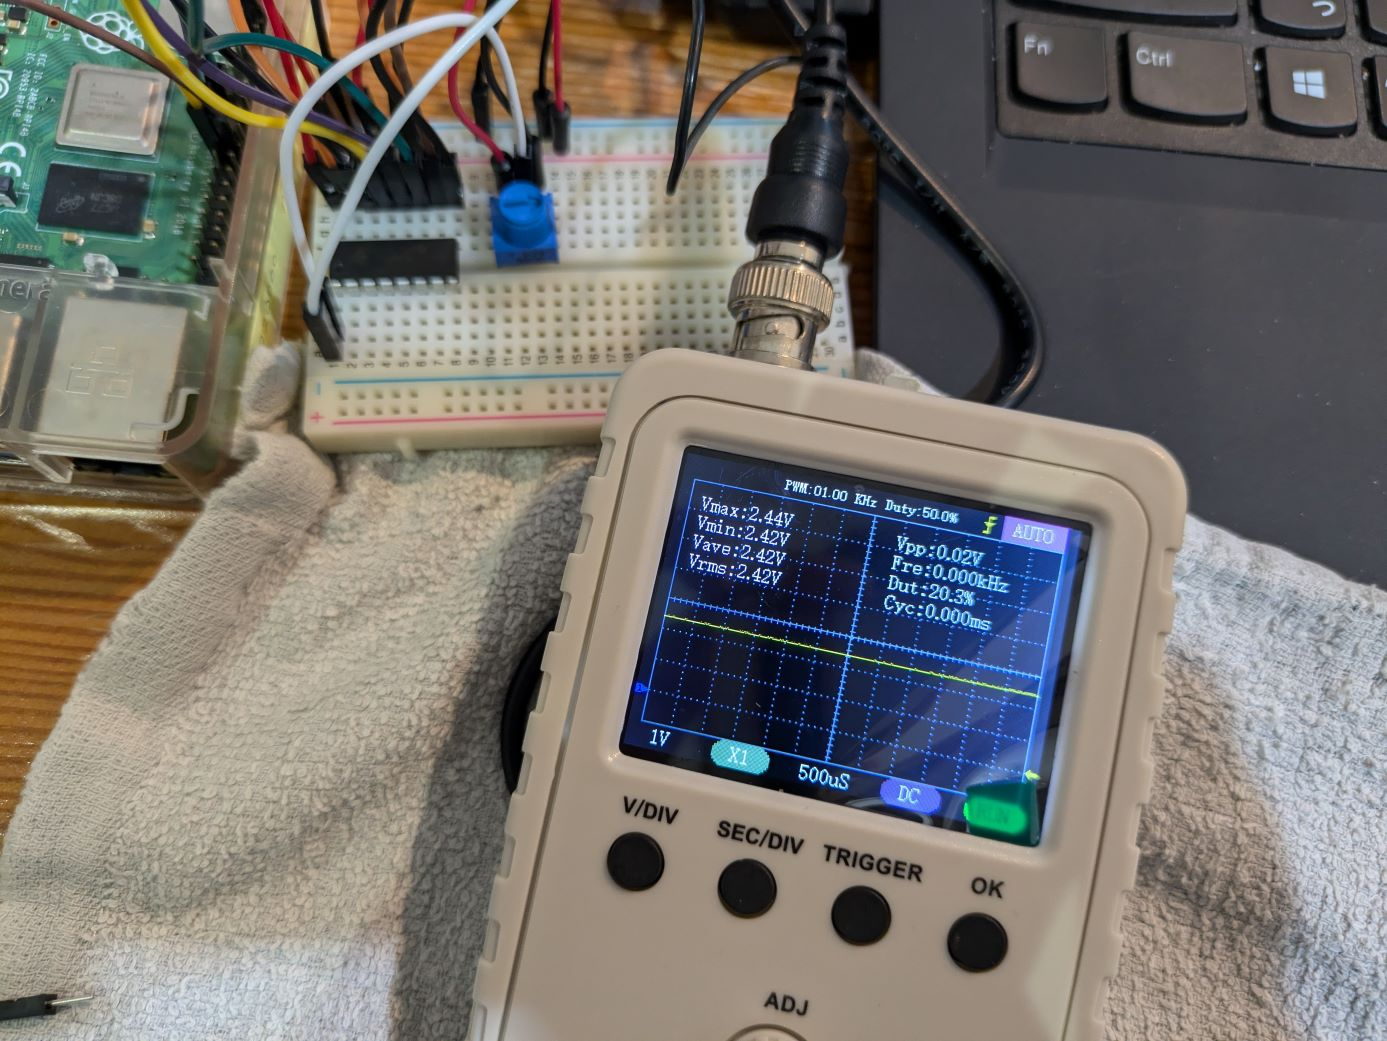
\includegraphics[width=\linewidth]{PXL_20241027_152756193_30.jpg}
    \caption{システム全景}
    \label{fig:system}
\end{figure}


\section{テスト}

本来ならば、実装におけるテスト項目は報告することではないが、
テストにより本実装の利用における制限事項が明らかになったので記述する。

シミュレータの制限事項
\begin{itemize}
    \item パラメータ$x$の上限と下限はそれぞれ10と0となる。
    \item 実行は10秒以上行ってはならない。これはバグではなく、繰り返し実行すると保持できるデータの上限が、、、。
\end{itemize}


\chapter{測定}\label{measurement}
Chapter\ref{implementation}で実装した
システムを
Raspberry Pi 4B (8GB)、
Windows PC (メモリ32GB)、
Azure上のサーバ(メモリ128GB+GPUどーん)で実行した。


\chapter{評価}\label{evaluation}

Chapter\ref{measurement}で得られたデータを評価する。
非常に多くのデータが取れた。


まず、
\begin{center}
    $x = 8$ \\
    $\sum_{i=1}^{10} x_i = f(x)$
\end{center}
の場合について考えてみる。



\chapter{考察}\label{discussion}

Chapter \ref{measurement}で得られたデータを
Chapter \ref{evaluation}で評価した結果、
及び、先行研究\cite{4065825}と合わせて、
本研究の到達地点について議論する。



%-------------------
%\bibliographystyle{plain} % 参考文献
\bibliographystyle{ieeetr} % 参考文献
\bibliography{myref} %
%-------------------

\begin{acknowledge}
本卒業研究を実施するにあたり、
\end{acknowledge}

\end{document}